%!TEX root = ../dissertation.tex

\chapter{The Algorithm} \label{cha:algorithm}

Having defined the OpenCog system and part of the implementation of the problem in the previous chapters, it is now possible to combine all the various modules and explain the functioning of the internal design and the main algorithm. \\

It is possible to divide the entire project into 6 phases: initial, perception, learning, request, search and results execution.  

\section{Initial Phase}\label{sec:init}

The initial phase concerns the initialization of the simulated environment. The framework used for the development and programming of the robot is the well-known ROS, Melodic version, and the Gazebo 9 system handles the simulation. \\
Therefore, the world as in Figure \ref{fig:env_2_named} is loaded into Gazebo. 
It consists of a robot manipulator with an attached camera, some fixed objects (such as tables, workbench and bins) and cubes, both with their AprilTags used for detection and semantic assignment. \\
Then, a server in C++ code is activated and the nodes of the ROS system for robot control and object perception become available for listening. \\
Finally, the main AtomSpace is created and the actions rules are loaded into it. 

\begin{figure} [h]
\centering
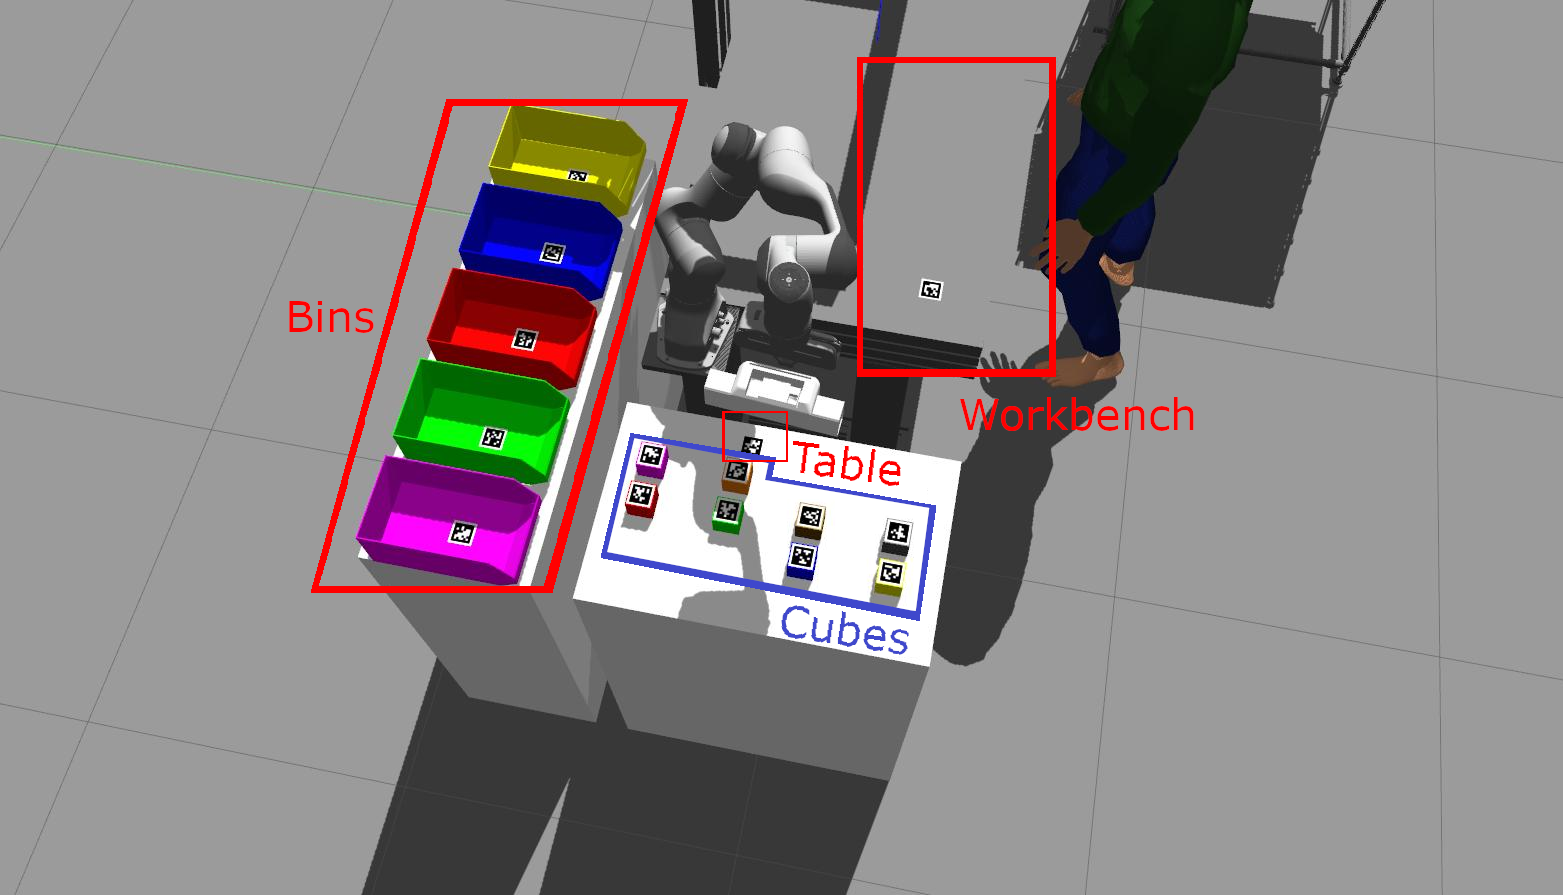
\includegraphics[width=1.0
\textwidth]{figures/Magistrale/env_objs}
\caption[Environment Components Description]{ In the red boxes are collected the objects that are considered fixed. Meanwhile, the blue box contains the remaining objects, represented by cubes.
\label{fig:env_2_named}}
\end{figure} 

\section{Perception Phase}\label{sec:perception}

The perception phase, like the remaining phases, is written in Python code and sends commands via a Python client to the C++ server mentioned above. These commands move the robot and allow it to scan its surrounding area for possible objects (related AprilTags are recognised), thanks to the camera attached to the top of it. \\
Of each AprilTag found, its associated semantic representation (i.e. English word describing the object, as well as the name of its relative ConceptNode, thus, for example: \enquote{table}, \enquote{workbench}, etc.) is returned by the server to the client, which in turn returns it to the main Python code that begins the initialization of the objects list, found in the environment.

\section{Learning Phase}\label{sec:learning}

The learning phase is used to provide additional information. \\
The perception algorithm is extremely simple and does not deal with information processing. Consequently, it is not able to distinguish an object from a fixed object or to infer that an object is placed on top of another. Surely, with a perception processing module all of this, and much more, could be managed. \\
However, this project shows the simplicity of integration and the potential of the learning with the OpenCog system. \\

This phase was created to tell the robot which objects are fixed, which are on top of others (fixed objects excluded) or which one is in the robot's hand. That is, to provide the necessary additional information, which the simple perception phase does not perceive, to describe the initial situation of the environment.
This is done by a module using NLP, consisting of the Relex2Logic OpenCog module and a post-processing phase. \\

Additional information is provided to the system via English sentences. \\
This module applies Relex2Logic to these sentences, creating the hypergraph describing them within a new empty AtomSpace (process explained in Section \ref{sec:r2l}).  \\
Next, the post-processing phase loads the rules presented in Section \ref{sec:NLP} and executes them within that AtomSpace. Those rules look for patterns corresponding to the possible information that the system might need and create summary atoms that can be easily used by the algorithm. Thus, from the results obtained by Relex2Logic, they infer atoms such as the ones shown in Section \ref{sec:env_atomese}, which are then added to the main AtomSpace. \\

Moreover, from the information learned in this phase, the \textit{clear} state atoms of the effectively free objects and the \textit{object} inheritance atoms of the non-fixed objects are created.  \\
Finally, the last atoms of the initial KB are added to the main AtomSpace. They are all possible simple combinations (without repetition) from the objects list taken two at a time (explained in Section \ref{sec:r2l}, too). \\
The main AtomSpace is now complete and fully describes the initial situation. 

\section{Request Phase}\label{sec:request}

The request phase behaves like the previous one, except for the aim. Whereas before, English sentences are used to give additional information, now new English sentences are requested to define the goal to be achieved. \\
In order to define the goal it is not necessary to describe the final complete arrangement of objects in the environment, but just the states of the objects one wants to achieve. \\
Thus, the same steps used in the learning phase are performed here. That is, the English sentences are processed to obtain the corresponding set of atoms that describes them. Then, these atoms are added to a goal list used by the algorithm to find a solution.

\section{Search Phase}\label{sec:search}

The search phase is the core of the algorithm and tries to achieve an arrangement of objects in which all atoms in the goal list are satisfied.
To find a solution, the AtomSpace of the final arrangement must contain every atom within the goal list. \\

Since each atom is unique in the AtomSpace, two AtomSpaces describing the same arrangement and state of objects have the same atoms, thus they are identical. 
Consequently, each possible arrangement of objects in the environment can be associated with one and only one AtomSpace, making it a de facto state of a Finite State Machine (FSM).
Moreover, each of the four actions available to the robot can be seen as a step of this FSM. 
Starting from a certain state, performing an action leads that state (i.e. that AtomSpace) into a new one. However, from each state, one or more actions can be performed and thus, one or more states can be reached. \\

One of the best ways to handle this structure is through a tree that has AtomSpaces as tree-nodes (to distinguish them from Nodes in Atomese) and available actions as tree-edges.
In addition, each tree-node has a label describing the action used, and on which objects, by its parent to create it.
In this way, each branch of the tree describes a different sequence of actions. They can be derived by starting with a solution tree-node and reading the labels of the parent tree-nodes backwards until the root, adding each label to a list. Finally, reversing the list.  \\

After the request phase, the root of the tree, containing the main AtomSpace and a \textit{NULL} label, is created. \\
Next, a search algorithm, based on the well-known Breadth-First Search (BFS) (more details in \cite{BFS-wiki, BFS}), expands the tree in search of a solution.

\subsection{BFS-Based Algorithm}\label{sec:bfs_search}

The BFS-based algorithm is recursive and accepts as arguments a tree-node and a variable, which limits the actions to be performed. \\
Following the rules of the problem (Secion \ref{cha:problem_description}), it is trivial to deduce that the actions alternate for each step of the algorithm.
That is, starting from the root:

\begin{enumerate} 
	\item If there exists an atom, within the AtomSpace contained in the root, that describes the \textit{in-hand} state of an object, then only \textit{Stack} and \textit{Putdown} actions can create children. Conversely, if there are no objects in hand, only the actions of \textit{Pickup} and \textit{Unstack} can. This is because the current state of the robot's hand limits the action used to go to the next state. If the hand is free, it can only grab an object, while if it is busy, it can only place the object down.

	\item From this first intuition, follows the one applicable to each step: given a certain tree-node, if the action \textit{Stack} or \textit{Putdown} created it, then the children of that node can only be created by \textit{Pickup} or \textit{Unstack} actions, otherwise vice versa.
\end{enumerate}

This is the reason why the BFS-algorithm has a variable as the second argument, it holds the action used to create the node in the first argument. \\
Trying all the actions at each step would also give the same result, but additional atoms would have to be added to the rule pattern to check whether the hand is free or busy.
Instead, following this design simplifies the rules, speeds up the algorithm and avoids unnecessary code execution.


\subsubsection{Termination Criteria of the BFS-Based Algorithm}\label{sec:term_criteria}

Some additional parameters are defined to limit and improve the search. As a result, it is possible to use 4 different searches:

\begin{enumerate}
	\item Search until a first solution is found
	\item Search restricted to a maximum number of iterations 
	\item Explore the whole tree
	\item Quick search
\end{enumerate}

The quick search finds a solution, decreasing the number of iterations in most situations.
As this type of problems suffers from combinatorial explosion\footnotemark{}, the number of tree-nodes grows exponentially as the tree expands.
\footnotetext{\url{https://en.wikipedia.org/wiki/Combinatorial_explosion}} \\
One way to reduce this expansion is to limit the available actions to only those that interact with one or more objects appearing in the goal list.
Many unnecessary actions are avoided, however this makes the algorithm incorrect, since the certainty of finding a solution is lost.
It still works well for most initial arrangements and goal lists and if it fails, the search in point 1 (which is correct if a solution exists, like searches in points 2 and 3) can be used. \\

Finally, a solution is found when all the atoms composing the goal list are within the AtomSpace of a tree-node. \\
Furthermore, the first solution found will certainly be the optimal solution, i.e. the solution that uses the minimum number of actions to go from the initial arrangement of objects to the goal one.
This is because for each tree-node, before being expanded, its AtomSpace is compared with the one of any tree-node belonging to its same branch.
If a match is found (i.e. they are identical), then the algorithm has come back to an arrangement of objects it has already encountered and thus, the sequence of subsequent actions would be a repetition of that associated with the matched tree-node. Consequently, the expansion of this tree-node ends.


\subsubsection{Steps of the BFS-Based Algorithm}\label{sec:step_search}

From the definitions above, it is now possible to list the steps that the BFS-based algorithm goes through. \\
The first recursive call has as arguments the root node (containing the main AtomSpace) and the variable defined according to the state of the hand.
Inside each call:

\begin{enumerate}
	\item It is checked if the maximum number of iterations is reached (in the case of limited search). As a consequence, the algorithm returns or continues.
	
	\item It is checked if the AtomSpace, contained in the tree-node argument, satisfies all the atoms in the goal list. If satisfied, this tree-node is added to the solution list and the algorithm returns or continues depending on the type of search.
	
	\item It is checked that the AtomSpace, contained in the tree-node argument, has not been encountered before. If encountered, this tree-node is not expanded and the algorithm moves on to the next one (Go back to point 1), otherwise its expansion begins.
	
	\item Now that the checks have been passed, the expansion of the tree-node argument occurs. \\
According to the variable argument, only two of the four actions can be executed.
Thus, from the AtomSpace of the current tree-node, two AtomSpace children (two copies of the parent) are created, one for each action. \\
Then, for each action (rule), the respective QueryLink without argument (i.e., the one that returns all possible objects that match the pattern; i.e., the objects on which that action can be performed), is executed within the AtomSpace assigned to it. \\
It is necessary to use AtomSpace copies because rule execution adds and removes atoms within AtomSpace and thus, modifies it. This means that executing a QueryLink without arguments modifies the AtomSpace as if the related action had been executed on all the matched objects at the same time, leading the AtomSpace into an incorrect state. \\
To summarise: 

	\begin{enumerate}
		\item AtomSpace copies are created
		\item Rules on generic objects are executed, one in each AtomSpace
		\item The objects, returned as solutions of the rules, correspond to the objects on which actions can be executed. They are stored in a list for each action.
		\item AtomSpace copies are cleaned up and deleted.
	\end{enumerate}

	\item Finally, for each object found, a copy of the AtomSpace of the tree-node argument is created again. Based on the list to which the object belongs, the corresponding action is executed in that AtomSpace, but this time using the QueryLink with the argument, which corresponds to that object. That is, the action is only executed on that object. \\
The resulting AtomSpaces are associated with new tree-nodes and become the children of the tree-node argument.
	
	\item At last, these new tree-nodes, obtained by executing the two actions available to each object on which they are applicable, are then added to a FIFO queue.
This queue is used for BFS. \\
The expansion of this tree-node is finished and the tree-node at the top of the queue is extracted and passed to a new recursive call of this algorithm, together with the variable describing the action used previously in its branch. 
\end{enumerate}


\section{Results Execution Phase}\label{sec:results_exec}

At the end of the search phase, the solution list contains the tree-nodes having an AtomSpace that satisfies all the atoms in the solution list.
As already explained in Section \ref{sec:search}, from each solution tree-node, a list containing a sequence of actions can be extracted.
If the solution list is not empty, then the first result corresponds to the optimal solution, otherwise either there is no solution or the search parameters need to be changed. \\
In conclusion, the optimal solution is sent from the client to the server, which will command the robot to perform each of those actions in sequence, thus achieving the required arrangement of objects.

\section{Practical Example}\label{sec:alg_example}

The following steps provide a simple practical example in order to clarify and contextualise the above phases.

\begin{enumerate}

	\item Initial Phase: \\
Loading environment (Ros, Gazebo, Relex2Logic Server, Cubes, AprilTags, etc.)

	\item Perception Phase: \\
Assume that four AprilTags are detected. Assume also that the AprilTags associate tree objects with a semantic meaning corresponding to parts of an industrial product to be assembled and the fourth with \enquote{workbench}. For simplicity in this example, the parts will be called \enquote{screw}, \enquote{bolt} and \enquote{washer}.

	\item Learning Phase: \\
The only additional information needed by the robot is: \enquote{The workbench is a fixed object.}. From this sentence the following atom will be extracted:
\begin{python}
	(InheritanceLink
		(ConceptNode "workbench")
		(ConceptNode "fixed-object"))
\end{python}

	\item Request Phase: \\
Assign an easy task: \enquote{The washer is on the screw. The bolt is on the washer.}.  From these sentences the following atoms will be extracted:
\begin{python}
	(EvaluationLink
		(PredicateNode "on")
		(ListLink
			(ConceptNode "washer")
			(ConceptNode "screw")))

	(EvaluationLink
		(PredicateNode "on")
		(ListLink
			(ConceptNode "bolt")
			(ConceptNode "washer")))
\end{python}

	\item Search Phase: \\
The Figure \ref{fig:BFS_1} shows the first steps of tree expansion using the BFS-based algorithm.
First, the hand is free, thus the algorithm will try to do \textit{Pickup} and \textit{Unstack} actions. Since \textit{screw}, \textit{bolt} and \textit{washer} are \textit{clear} objects, the first iteration of the algorithm will create 3 tree-nodes corresponding to the initial object arrangement (i.e., the arrangement of the root), except the one to which \textit{Pickup} is performed. \\
The \textit{workbench} is a fixed object, thus it is not found as a solution of \textit{Pickup}, moreover the action \textit{Unstack} returns an empty result because there are no stacked objects\footnotemark{}.
\footnotetext{The objects are actually stacked relative to the workbench. However, this fixed object can be considered as the initial one and therefore one can ignore the stacks and use actions of \textit{Pickup} and \textit{Putdown}, alternatively the stacks can be added as information during the learning phase and consequently, actions of \textit{Stack} and \textit{Unstack} will be used instead.}
\\Subsequently, these tree-nodes are analysed following the order corresponding to the blue numbers in the figure. None of them is a solution tree-node or has an AtomSpace already encountered, thus, their children are created. \\
Tree-node number 4 is obtained by making \textit{Pickup} of A and then \textit{Putdown} of the same, so its AtomSpace will correspond to the one of the root. Consequently, its expansion ends. \\
The expansions continue until the yellow tree-node is reached, which has an AtomSpace containing all the atoms in the goal list. Therefore, a solution is found and the search ends (Quick search).

\begin{figure} [h]
\centering
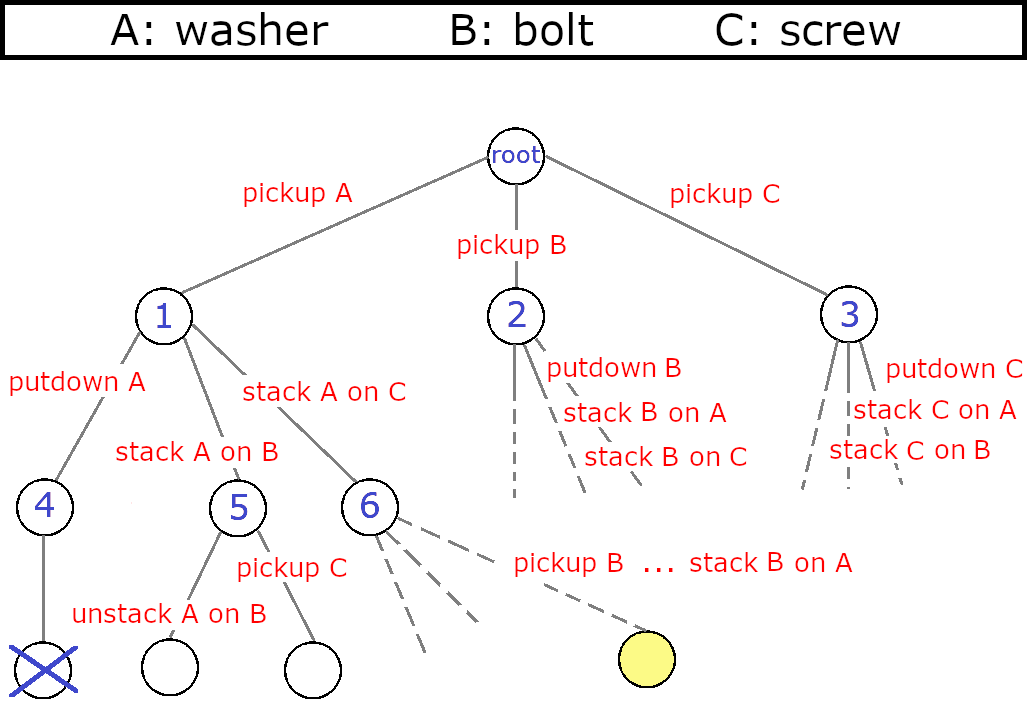
\includegraphics[width=1.0
\textwidth]{figures/Magistrale/BFS_1_blue}
\caption[BFS Example]{Graph describing the expansion of the tree of the practical example.  \\
Each node contains an AtomSpace and each edge describes an action. \\
Each AtomSpace at an internal node is unique among all those contained in its branch. With the exception of AtomSpaces at leaf nodes that either already exist within its own branch (node marked with a blue X) or are a solution (yellow node). \\
The order of node expansion is shown by the sequence of numbers within them and follows the order of the BFS. \\
The legend on the top simplifies the labels in the tree by using the letters A, B, C instead of names used in the algorithm. 
\label{fig:BFS_1}}
\end{figure} 

The sequence of actions from the initial arrangement to the goal arrangement can easily be read from the tree-edges, going up the branch from the yellow tree-node to the root.
	
	\item Results Execution Phase: \\
The following sequence of actions will be performed by the robot, satisfying the initial request:
\begin{python}
	- Pickup washer
	- Stack washer on screw
	- Pickup bolt
	- Stack bolt on washer
\end{python}
\end{enumerate}